\section{Solution Architecture}

In this section, we present the client-server architecture chosen for Credix, which clearly separates the front-end developed with Flutter from the back-end implemented with Spring Boot. This architectural choice perfectly adapts to our context, offering flexibility, scalability, and a better distribution of responsibilities. We will then detail the main components and layers of the application, for both the front-end and the back-end.

\subsection{Justification of RESTful Web Services Architecture}

To ensure better scalability, a clear separation of responsibilities, and the possibility of independent evolutions, we have adopted a client-server architecture based on RESTful Web Services. The front-end developed with Flutter communicates via HTTP with a Spring Boot back-end exposing REST APIs. The main advantages of this choice are:

\begin{itemize}
    \item \textbf{Layer Decoupling:} The front-end (Flutter) communicates via HTTP with a Spring Boot back-end, which exposes REST APIs. This allows the user interface to evolve independently of the business logic.
    \item \textbf{Service Reusability:} Each core component (e.g., authentication, payment processing, corporate credit management, fraud detection) becomes a distinct, reusable service.
    \item \textbf{Fine-grained Scalability:} Critical services (e.g., real-time payment validation, fraud engine) can be scaled autonomously based on load, without impacting the other services.
    \item \textbf{Third-party Service Integration:} We seamlessly integrate with external services, notably ASM POS APIs for barcode scanning and validation, without additional complexity in the core business code.
    \item \textbf{Resilience and Maintenance:} In case of a service failure (e.g., a specific payment gateway issue), the rest of the application continues to function, and each service can be updated or redeployed separately, ensuring high availability.
\end{itemize}

\subsection{Overview}
Our architecture distinguishes three main layers:

\begin{itemize}
    \item \textbf{Front-end (Flutter):} The mobile application responsible for the User Interface (UI), managing states via BLoC, and making API calls to the backend.
    \item \textbf{Back-end (Spring Boot):} The REST APIs exposing business endpoints, orchestrating calls to the database (PostgreSQL) and third-party services (ASM POS).
    \item \textbf{Third-party Services:} Primarily ASM POS APIs, which integrate via HTTP for real-time payment validation and settlement synchronization.
\end{itemize}

\subsection{Backend Components}

The Spring Boot back-end is structured into three main layers:

% Updated to use new backend architecture diagram
\begin{figure}[H]
    \centering
    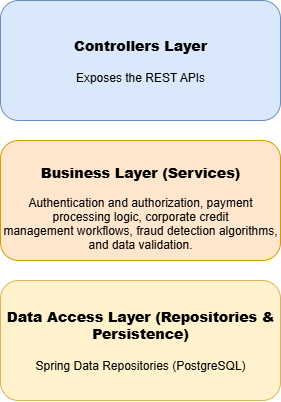
\includegraphics[width=0.6\textwidth]{images/backend_architecture_diagram.png}
    \caption{Credix Backend Architecture}
    \label{fig:backend_architecture}
\end{figure}

\begin{itemize}
    \item \textbf{Controllers Layer:} Exposes the REST APIs for the Flutter front-end and handles incoming requests from ASM POS systems. It acts as the entry point for all client and third-party interactions.
    \item \textbf{Business Layer (Services):} Implements the core business rules, including user authentication and authorization, payment processing logic, corporate credit management workflows, fraud detection algorithms, and data validation.
    \item \textbf{Data Access Layer (Repositories \& Persistence):} Defines Spring Data interfaces (e.g., JPA Repositories) and manages persistence in the PostgreSQL database for all application data, such as user profiles, transaction records, corporate accounts, and audit logs.
\end{itemize}

\subsection{Frontend Components}

The Flutter client follows Clean Architecture principles with a clear five-layer decomposition, promoting maintainability, testability, and separation of concerns:

% Updated to use new frontend architecture diagram
\begin{figure}[H]
    \centering
    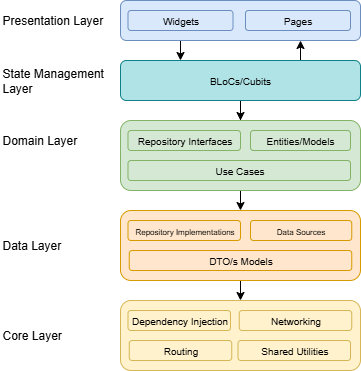
\includegraphics[width=0.7\textwidth]{images/frontend_architecture_diagram.png}
    \caption{Credix Frontend Architecture - Clean Architecture Pattern}
    \label{fig:frontend_architecture}
\end{figure}

\begin{itemize}
    \item \textbf{Presentation Layer (Pages \& Widgets):} Contains all UI components organized by features (authentication, wallet, transactions, barcode scanning, etc.). This layer focuses purely on rendering the user interface and handling user interactions. Each feature includes dedicated pages and reusable widgets that display data and capture user input.
    
    \item \textbf{State Management Layer (BLoCs/Cubits):} Acts as an intermediary between the UI and business logic, implementing the BLoC (Business Logic Component) pattern. This layer handles user events, manages application state, and emits new states to update the UI reactively. Each feature has its dedicated BLoC (AuthBloc, WalletBloc, TransactionBloc, etc.) ensuring clean separation of presentation logic.
    
    \item \textbf{Domain Layer (Business Logic):} Defines repository interfaces, entities, and use cases that encapsulate core business rules. This layer is completely independent of external frameworks and contains the pure business logic of the application. It defines contracts through repository interfaces and implements business validation rules, ensuring high testability and maintainability.
    
    \item \textbf{Data Layer (Repository Implementations):} Implements the repository interfaces defined in the domain layer and manages all data operations. This layer handles multiple data sources including remote APIs (via Dio HTTP client), local storage (SharedPreferences, SQLite), and manages data transformation between external formats (DTOs) and domain models.
    
    \item \textbf{Core Layer (Shared Infrastructure):} Provides shared utilities and infrastructure components used across all features. This includes dependency injection configuration (Injectable/GetIt), networking setup (Dio interceptors, API configuration), routing management (Auto Route), application theming, constants, extensions, and common widgets shared between features.
\end{itemize}

\subsection{Continuous Integration and Deployment (CI/CD)}

Credix leverages automated CI/CD pipelines to ensure rapid, reliable, and consistent delivery of software updates for both its backend and frontend components.

% Updated to use new CI/CD pipeline diagram
\begin{figure}[H]
    \centering
    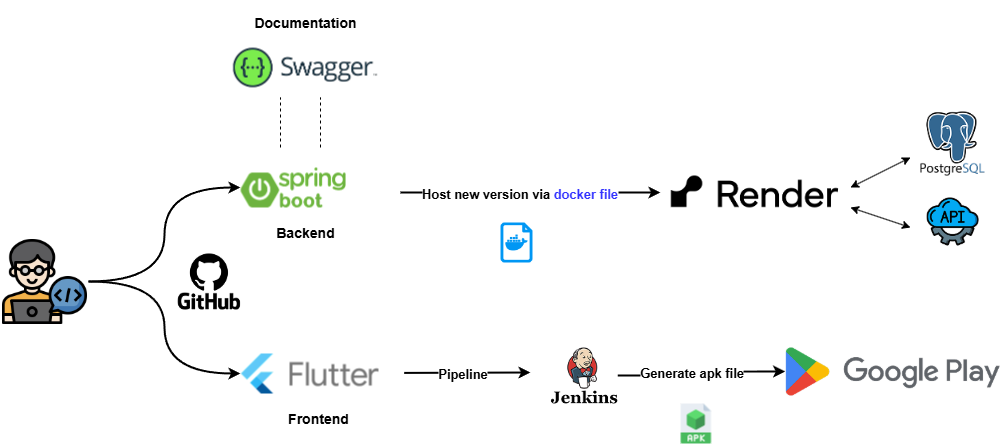
\includegraphics[width=\textwidth]{images/ci_cd_pipeline_diagram.png}
    \caption{CI/CD Pipeline Architecture}
    \label{fig:cicd_pipeline}
\end{figure}

Credix leverages automated CI/CD pipelines to ensure rapid, reliable, and consistent delivery of software updates for both its backend and frontend components.

\begin{itemize}
    \item \textbf{Back-end (Spring Boot):}
    When a developer pushes code to the backend's GitHub repository, a GitHub Actions pipeline is immediately triggered. This pipeline builds a new Docker image of the Spring Boot service, runs automated tests, and then deploys the updated application to the production environment without manual intervention. This ensures that new backend features and bug fixes are continuously delivered and available.

    \item \textbf{Front-end (Flutter):}
    Similarly, as soon as a front-end developer pushes their modifications to GitHub, a dedicated GitHub Actions pipeline for Flutter executes. This pipeline compiles the mobile application, runs automated tests, generates an APK for internal testing phases, and an AAB (Android App Bundle) for the Google Play Store. These artifacts are then stored in the project's "Releases" section. This automation allows for rapid publication of new versions of the Credix mobile application to Google Play, while minimizing errors associated with manual deployment processes.
\end{itemize}
